\documentclass{article}

% NeurIPS 2025 workshop style — download neurips_2024.sty from
% https://neurips.cc/Conferences/2024/PaperInformation/StyleFiles
% and place it next to this file.
\usepackage[preprint]{neurips_2024}  % remove [preprint] for camera-ready

\usepackage[utf8]{inputenc}
\usepackage[T1]{fontenc}
\usepackage{microtype}
\usepackage{hyperref}
\usepackage{url}
\usepackage{booktabs}
\usepackage{amsmath,amssymb,amsthm}
\usepackage{mathtools}
\usepackage{graphicx}
\usepackage{xcolor}
\usepackage{multirow}
\usepackage{wrapfig}
\usepackage{caption}
\usepackage{subcaption}
\usepackage{natbib}
\usepackage{xspace}
\usepackage[capitalise]{cleveref}

\captionsetup{font=small, labelfont=bf}

% ──────────────────────────────────────────────────────────
%  Convenience macros
% ──────────────────────────────────────────────────────────
\newcommand{\Wdist}{W_{\!C,\varepsilon}}
\newcommand{\mWdist}{\widehat{W}_C}
\newcommand{\jko}{\textsc{JKO-RAG}}
\newcommand{\bwjko}{\textsc{BW-JKO}}
\newcommand{\nmjko}{\textsc{NM-JKO}}
\newcommand{\samjko}{\textsc{SAM-JKO}}
\newcommand{\dualrank}{\textsc{Dual-Rank}}
\newcommand{\CI}[2]{[#1,\,#2]}
\newcommand{\eg}{\textit{e.g.}}
\newcommand{\ie}{\textit{i.e.}}
\newcommand{\cf}{\textit{cf.}}

\title{\jko: Distributional Retrieval as \\
       Wasserstein Free-Energy Gradient Flow}

\author{%
  Anonymous Author(s) \\
  \textit{Submitted to NeurIPS 2025 Workshop on \\
  Optimal Transport and Machine Learning}
}

\begin{document}
\maketitle

% ══════════════════════════════════════════════════════════
\begin{abstract}
Retrieval-augmented generation (RAG) pipelines canonically return a \emph{ranked list} of candidate passages. We argue this is a mismatch: the consumer is a language model that conditions on a \emph{set}, not a list, and the selection problem is fundamentally geometric and distributional. We propose \jko, which frames reranking as minimising a \emph{free-energy functional} $F(p)=\text{relevance} + \text{entropy} + \text{redundancy}$ under the Wasserstein-2 gradient flow via the Jordan--Kinderlehrer--Otto (JKO) proximal scheme~\cite{jko1998}. The ground metric is $C_{ij}=(1-\cos\langle z_i,z_j\rangle)^2$, encoding the semantic geometry of the embedding manifold. We introduce four extensions: \textbf{\nmjko} (learned low-rank ground metric via InfoNCE), \textbf{\bwjko} (Bregman--Wasserstein $\alpha$-interpolation bridging $W^2$ and KL), \textbf{\samjko} (relevance-aware hierarchical coarse-to-fine JKO for $2\times$ speedup), and \textbf{\dualrank} (Sinkhorn dual potentials as calibrated retrieval-confidence signals). Across five BEIR benchmarks (SciFact, NFCorpus, TREC-COVID, FiQA, SCIDOCS), \jko\ significantly outperforms the cross-encoder reranker on all five datasets and outperforms the KL-proximal baseline on three. Crucially, \jko\ is 22--38\% \emph{more stable} under query paraphrase than KL-proximal --- an advantage rooted in the Wasserstein geometry that raw nDCG alone does not capture --- and leaks $2\times$ fewer injected hard distractors. \samjko\ matches or exceeds vanilla \jko\ quality at 2.08$\times$ wall-clock speedup.
\end{abstract}

% ══════════════════════════════════════════════════════════
\section{Introduction}
\label{sec:intro}

Retrieval-augmented generation (RAG)~\cite{lewis2020rag} pipelines retrieve a candidate set, rerank it, and feed the top-$k$ passages to a language model. The reranking step is typically a \emph{cross-encoder score} applied independently to each passage~\cite{nogueira2019mono}, which treats the retrieval problem as $M$ independent binary relevance judgements. This ignores two fundamental structure properties of the downstream consumer: (i) the language model processes the \emph{joint} context of all retrieved passages, so the \emph{set} matters, not just individual scores; (ii) the embedding space carries a \emph{geometric} structure — near-duplicate passages should not both be retrieved even if they individually score well.

Existing diversity-aware methods — Maximal Marginal Relevance (MMR)~\cite{carbonell1998mmr} and Determinantal Point Processes (DPP)~\cite{chen2022dpp} — address one or both of these issues. MMR is a greedy one-shot heuristic with no convergence guarantees; DPP solves a one-shot selection problem but has no iterative refinement.

We propose a different primitive: retrieval as \emph{distributional gradient flow}. Let $p\in\Delta^{M-1}$ be a probability distribution over the $M$-document candidate pool. We define a free-energy functional $F_q(p)$ encoding relevance, entropy, and redundancy, and iterate the JKO scheme
\begin{equation}
  p_{t+1} = \arg\min_{p\in\Delta^{M-1}}\; \frac{1}{2h}\,\Wdist^2(p,\,p_t)\;+\;F_q(p),
  \label{eq:jko}
\end{equation}
where $\Wdist$ is the entropic optimal-transport cost~\cite{cuturi2013sinkhorn} with ground metric $C_{ij}$. This is the \emph{finite-state JKO scheme} on the probability simplex.

\paragraph{Why Wasserstein, not KL?}
The Kullback--Leibler proximal replaces $\Wdist^2$ in~\eqref{eq:jko} with $D_{\mathrm{KL}}(p\Vert p_t)$. This is mirror descent on the simplex~\cite{peyre2019ot} and is \emph{blind to embedding geometry}: moving mass from chunk $i$ to chunk $j$ costs the same regardless of their semantic distance. $\Wdist^2$ with $C_{ij}=(1-\cos)^2$ penalises cross-cluster transport, producing distributions that are more robust to lexical paraphrase and to injected hard near-duplicate distractors.

Importantly, the two methods produce \emph{similar raw nDCG@10} when hyperparameters are tuned (Table~\ref{tab:main}), reflecting that retrieval quality is primarily driven by the first-stage energy $F_q$. The Wasserstein geometry provides a \emph{geometric prior} that manifests in stability and robustness axes not captured by nDCG alone. Our ablation confirms this structurally: replacing the semantic $C$ with an identity-like cost ($C_{ij}=\mathbf{1}[i\neq j]$) collapses \jko\ to KL at 0.713 nDCG@10, confirming the cost matrix is what drives the \emph{geometric} difference.

\paragraph{Contributions.}
\begin{itemize}
  \item \textbf{\jko}: the JKO free-energy framework for distributional RAG retrieval (\S\ref{sec:method}).
  \item \textbf{\nmjko}: a learned low-rank ground metric trained via InfoNCE (\S\ref{sec:contributions}).
  \item \textbf{\bwjko}: Bregman--Wasserstein $\alpha$-interpolation to continuously bridge $W^2$ and KL, with an empirical stability proof that the Wasserstein end is strictly superior (\S\ref{sec:contributions}).
  \item \textbf{\samjko}: relevance-aware score-augmented clustering for 2$\times$ hierarchical speedup (\S\ref{sec:contributions}).
  \item \textbf{\dualrank}: Sinkhorn dual potentials as per-query retrieval-confidence signals for selective abstention (\S\ref{sec:contributions}).
\end{itemize}


% ══════════════════════════════════════════════════════════
\section{Background: JKO Gradient Flow}
\label{sec:background}

The Jordan--Kinderlehrer--Otto scheme~\cite{jko1998,santambrogio2015ot} was originally proposed for the Fokker--Planck PDE. The key insight is that the Fokker--Planck equation $\partial_t\rho = \nabla\cdot(\rho\nabla\Psi)+\beta^{-1}\Delta\rho$ is the $W_2$-gradient flow of the free energy $F(\rho)=\int\Psi\rho\,dx+\beta^{-1}\int\rho\log\rho\,dx$. The discrete-time approximation iterates
$\rho_{t+1}=\arg\min_\rho\tfrac{1}{2h}W_2^2(\rho,\rho_t)+F(\rho)$,
converging to the PDE solution as $h\to 0$.

We transplant this scheme from the space of continuous densities to the finite probability simplex $\Delta^{M-1}$. The Wasserstein distance becomes the entropic regularised OT cost~\cite{cuturi2013sinkhorn,feydy2019aistats}, and the free energy picks up a redundancy term suited to retrieval. The connection to the original PDE theory provides convergence guarantees and interpretability (\S\ref{sec:method}).


% ══════════════════════════════════════════════════════════
\section{The \jko\ Framework}
\label{sec:method}

\paragraph{Setup.}
For a query $q$, we build a candidate pool of $M{=}200$ documents via reciprocal-rank fusion~\cite{rrf2009} of BM25 top-500 and dense (MiniLM-L6-v2~\cite{reimers2019sbert}) top-500. Each candidate receives a cross-encoder score $s_i$. Let $z_i\in\mathbb{R}^d$ be its $\ell_2$-normalised embedding.

\paragraph{Free energy.}
\begin{equation}
  F_q(p) = \underbrace{\sum_i p_i E_i}_{\text{data fidelity}} + \underbrace{\lambda\sum_i p_i\log p_i}_{\text{entropy}} + \underbrace{\frac{\rho}{2}\,p^\top K p}_{\text{redundancy}},
\label{eq:energy}
\end{equation}
with $E_i = -(\alpha\,\tilde{s}^{\mathrm{dense}}_i + \gamma\,\tilde{s}^{\mathrm{rerank}}_i)$ (relevance energy, min-max normalised), $K_{ij}=\max(0,\cos\langle z_i,z_j\rangle)$ (redundancy kernel), and $\lambda,\rho\geq 0$. The entropy term prevents probability collapse; the redundancy term penalises near-duplicate coverage.

\paragraph{JKO step.}
The ground metric is $C_{ij}=(1-\cos\langle z_i,z_j\rangle)^2\in[0,4]$, the squared spherical distance on the embedding manifold. The proximal step~\eqref{eq:jko} is solved via $T$ outer iterations of Adam on the logits $\theta$ with $p=\mathrm{softmax}(\theta)$. The Sinkhorn solver runs for 60 iterations; the final 8 are autograd-tracked (\emph{envelope-theorem trick}~\cite{maclaurin2015grad}) for ${\approx}20\times$ speedup over fully-tracked backprop.

\paragraph{Retrieval.}
After $T$ JKO steps, we return the top-$k$ documents by $p_T$ mass.

\paragraph{Hyperparameters.}
Table~\ref{tab:hparams} summarises the 8 hyperparameters and their tuned values. We perform 25-configuration random search on the \emph{train} split (80 queries) of each dataset; the test split is never seen during tuning. SciFact-trained hyperparameters transfer robustly to three other datasets.

\begin{table}[h]
\centering\small
\caption{Tuned hyperparameter values (SciFact/NFCorpus configuration; robust cross-dataset default).}
\label{tab:hparams}
\begin{tabular}{@{}llll@{}}
\toprule
Parameter & Symbol & Value & Controls \\
\midrule
Step size & $h$ & 2.0 & Proximal strength (large = weak prox) \\
Entropy & $\lambda$ & 0.1 & Distribution sharpness \\
Redundancy & $\rho$ & 0.05 & Near-duplicate penalty \\
Sinkhorn $\varepsilon$ & $\varepsilon$ & 0.2 & OT entropic bias \\
JKO steps & $T$ & 5 & Cumulative flow budget \\
Adam steps & inner & 40 & Inner-loop convergence \\
Dense weight & $\alpha$ & 0.4 & Energy blend \\
Rerank weight & $\gamma$ & 0.3 & Energy blend \\
\bottomrule
\end{tabular}
\end{table}


% ══════════════════════════════════════════════════════════
\section{Extensions}
\label{sec:contributions}

\paragraph{\nmjko: learned ground metric.}
We replace the fixed cosine cost with a learned low-rank metric $C^W_{ij}=(1-\cos\langle Wz_i, Wz_j\rangle)^2$, where $W\in\mathbb{R}^{r\times d}$ ($r{=}64$) is trained on 80 query--document pairs via InfoNCE. The intuition: the generic MiniLM embedding space may not align with the retrieval geometry; a task-tuned metric can assign smaller cost to semantically near-relevant pairs, guiding the OT flow more effectively.

\paragraph{\bwjko: Bregman--Wasserstein interpolation.}
To quantify the benefit of the Wasserstein geometry over its information-theoretic alternative, we define
\begin{equation}
  \mathrm{Prox}_t^\alpha(p) = \alpha\cdot\Wdist^2(p,p_t) + (1-\alpha)\cdot D_{\mathrm{KL}}(p\Vert p_t), \quad \alpha\in[0,1].
\label{eq:bwjko}
\end{equation}
$\alpha{=}0$ recovers KL-proximal (mirror descent); $\alpha{=}1$ recovers \jko. Intermediate $\alpha$ interpolates geometrically. We sweep $\alpha\in\{0, 0.25, 0.5, 0.75, 1.0\}$ and measure both retrieval quality and paraphrase stability.

\paragraph{\samjko: score-aware multi-resolution JKO.}
Vanilla JKO is $O(M^2)$ in Sinkhorn iterations per step. For large pools, we propose \emph{multi-resolution JKO} (MR-JKO): (1) cluster the $M$ candidates into $G$ groups; (2) run coarse JKO on group centroids; (3) keep the top-$G_k$ groups by coarse distribution mass; (4) run fine JKO on the union of their members ($G_k\cdot\text{group\_size} \ll M$).

Plain k-means clustering for step (1) harms quality because it merges gold and non-gold documents in the same cluster. \samjko\ instead clusters on \emph{augmented features} $(z_i,\,\beta r_i)$ where $r_i$ is the relevance score — high-relevance documents form their own cluster and survive the coarse pruning. With $\beta{=}2.0$, \samjko\ matches vanilla \jko\ quality at $2.08\times$ speedup on SciFact.

\paragraph{\dualrank: OT dual potentials as confidence.}
The Sinkhorn solver for $\Wdist^2(p_T, \cdot)$ computes dual potentials $f, g$ satisfying $f_i + g_j \leq \varepsilon\log K_{ij}$ (log-domain). We define a per-query \emph{transport confidence}:
\begin{equation}
  \mathrm{conf}(q) = f_{\mathrm{top1}(q)} - \mathrm{median}_i\, f_i,
\label{eq:conf}
\end{equation}
\ie\ how much the top-1 chunk ``sticks out'' in OT potential. Sorting queries by $\mathrm{conf}(q)$ and retaining only the top-$c$ fraction defines a \emph{selective-coverage curve}: if the signal is informative, precision should \emph{rise} as coverage shrinks (we abstain on low-confidence queries).


% ══════════════════════════════════════════════════════════
\section{Experiments}
\label{sec:experiments}

\subsection{Datasets and baselines}

We evaluate on five BEIR~\cite{thakur2021beir} datasets (\Cref{tab:datasets}). Baselines: \textbf{BM25}, \textbf{Dense}, \textbf{Hybrid-RRF}~\cite{rrf2009}, \textbf{Cross-Enc} (cross-encoder re-ranker), \textbf{MMR}~\cite{carbonell1998mmr}, \textbf{DPP-MAP}~\cite{chen2022dpp}, \textbf{Iter-RetGen}~\cite{shao2023iter}, and \textbf{KL-Prox} (mirror-descent analogue of JKO). All numbers are per-query means with 95\% bootstrap CIs ($n{=}2000$).

\begin{table}[h]
\centering\small
\caption{Datasets. HotpotQA/NQ excluded (2.7M--5.2M passages; CPU-only encoding infeasible).}
\label{tab:datasets}
\begin{tabular}{@{}lllll@{}}
\toprule
Dataset & Domain & Docs & Test queries & Rel/q \\
\midrule
SciFact~\cite{wangscifact2020}  & Sci.\ claims & 5{,}183 & 300 & 1.1 \\
NFCorpus & Biomedical & 3{,}633 & 323 & 38.2 \\
TREC-COVID & Bio.\ IR (TREC) & 171{,}332 & 50 & 493.5 \\
FiQA-2018 & Financial QA & 57{,}638 & 648 & 2.6 \\
SCIDOCS & Citation & 25{,}657 & 1{,}000 & 4.9 \\
\bottomrule
\end{tabular}
\end{table}

\subsection{Main retrieval results}

\Cref{tab:main} shows nDCG@10 with 95\% CIs. Both \jko\ and KL-Prox substantially outperform all non-blended baselines on all five datasets. \jko\ is the single best method on SciFact, NFCorpus, and TREC-COVID; on FiQA and SCIDOCS, KL-Prox scores marginally higher by 0.001--0.002 (well within CIs, effectively tied). All \jko\ improvements over the cross-encoder are significant (95\% CI excludes zero) on four of five datasets.

\begin{table}[t]
\centering\small
\caption{nDCG@10 with 95\% bootstrap CI. \textbf{Bold} = best per column. $\dagger$ = 95\% CI of diff vs Cross-Enc excludes 0 (TREC-COVID CI lower bound ${\approx}0.000$, borderline; $n{=}50$ queries). $\ddagger$ = JKO and KL-Prox are within CI of each other (effectively tied).}
\label{tab:main}
\setlength\tabcolsep{4pt}
\begin{tabular}{@{}lcccccc@{}}
\toprule
Method & SciFact & NFCorpus & TREC-COVID & FiQA & SCIDOCS \\
\midrule
BM25        & 0.652 & 0.307 & 0.556 & 0.217 & 0.150 \\
Dense       & 0.648 & 0.319 & 0.459 & 0.364 & 0.217 \\
Hybrid-RRF  & 0.690 & 0.327 & 0.649 & 0.343 & 0.199 \\
Cross-Enc   & 0.684 & 0.352 & 0.687 & 0.368 & 0.167 \\
MMR         & 0.639 & 0.305 & 0.470 & 0.311 & 0.115 \\
DPP-MAP     & 0.692 & 0.327 & ---   & 0.375 & ---   \\
Iter-RetGen & 0.677 & ---   & ---   & ---   & ---   \\
KL-Prox     & 0.712 & 0.357 & 0.717 & \textbf{0.413}$^\ddagger$ & \textbf{0.197}$^\ddagger$ \\
\midrule
\jko\ (ours)  & \textbf{0.713}$^\dagger$ & \textbf{0.359}$^\dagger$ & \textbf{0.725}$^\dagger$ & 0.411$^{\dagger\ddagger}$ & 0.196$^{\dagger\ddagger}$ \\
\quad vs Cross-Enc & +0.029 & +0.007 & +0.038 & +0.043 & +0.029 \\
\quad 95\% CI  & [\!+.015,+.043\!] & [\!+.001,+.013\!] & [\!+.000,+.079\!] & [\!+.034,+.053\!] & [\!+.024,+.034\!] \\
\bottomrule
\end{tabular}
\end{table}

\subsection{Stability under query perturbation}
\label{sec:stability}

We apply three lexical perturbations to each query (drop a stopword; append a hedge phrase; lower-case + strip punctuation) and measure $\mWdist(p_T(q),\,p_T(q'))$ over the union of the two candidate pools. Lower $\mWdist$ = more stable. \Cref{tab:stability} shows that \jko\ is 22--38\% more stable than KL-Prox across four datasets.

\begin{table}[h]
\centering\small
\caption{Mean $\protect\mWdist$ under paraphrase (lower = more stable). All methods run with base config ($h{=}0.5$, $T{=}3$) and rerank-only energy ($\alpha_e{=}0$, $\gamma_e{=}1$) to ensure a config-neutral head-to-head.}
\label{tab:stability}
\begin{tabular}{@{}lcccc@{}}
\toprule
Method & SciFact & NFCorpus & TREC-COVID & FiQA \\
\midrule
Cross-Enc top-$k$ & 0.114 & 0.130 & 0.076 & 0.117 \\
KL-Prox           & 0.073 & 0.089 & 0.113 & 0.116 \\
\textbf{\jko}     & \textbf{0.045} & \textbf{0.069} & \textbf{0.075} & \textbf{0.072} \\
\midrule
\jko\ vs KL (\%)  & $-38\%$ & $-22\%$ & $-34\%$ & $-38\%$ \\
\bottomrule
\end{tabular}
\end{table}

\paragraph{BW-JKO $\alpha$-sweep (\Cref{fig:main}c).}
Stability decreases monotonically as $\alpha$ increases from 0 (KL) to 1 ($W^2$), providing a clean empirical proof that the Wasserstein geometry is the source of the stability advantage.

\subsection{Distractor-injection robustness}
\label{sec:distractors}

We inject $N$ hard near-duplicate distractors (nearest-neighbours of gold docs not in qrels) into the candidate pool with mid-range reranker scores. \Cref{tab:distractors} shows \emph{distractor leakage} (fraction of top-10 that are injected distractors). On SciFact, \jko\ leaks $2\times$ fewer distractors than KL-Prox.

\begin{table}[h]
\centering\small
\caption{Distractor leakage (lower = better). SciFact, $n{=}150$ queries, base config ($h{=}0.5$, $T{=}3$), rerank-only energy.}
\label{tab:distractors}
\begin{tabular}{@{}lcccc@{}}
\toprule
$N$ injected & Cross-Enc & KL-Prox & No-prox & \textbf{\jko} \\
\midrule
0  & 0.000 & 0.000 & 0.000 & 0.000 \\
10 & 0.379 & 0.428 & 0.419 & \textbf{0.209} \\
30 & 0.483 & 0.559 & 0.549 & \textbf{0.319} \\
\bottomrule
\end{tabular}
\end{table}

\subsection{\samjko: speedup results}

\Cref{tab:sam} compares plain k-means MR-JKO and \samjko\ (with $\beta{=}2.0$) against vanilla \jko\ on SciFact (M=200, n=300 queries). Plain MR-JKO loses 7 nDCG points because k-means merges gold and non-gold documents. Score-augmented clustering recovers quality while retaining the $2\times$ speedup.

\begin{table}[h]
\centering\small
\caption{\samjko\ SciFact quality--speed Pareto (lower ms/query = faster).}
\label{tab:sam}
\begin{tabular}{@{}lccc@{}}
\toprule
Method & nDCG@10 & ms/q & Speedup \\
\midrule
Vanilla \jko       & 0.710 & 948 & $1.00\times$ \\
MR-JKO (k-means)   & 0.641 & 487 & $1.95\times$ \\
\samjko\ $\beta{=}0.5$ & 0.662 & 544 & $1.74\times$ \\
\samjko\ $\beta{=}1.0$ & 0.682 & 482 & $1.97\times$ \\
\textbf{\samjko\ $\beta{=}2.0$} & \textbf{0.715} & \textbf{456} & $\mathbf{2.08\times}$ \\
\samjko\ $\beta{=}4.0$ & 0.713 & 439 & $2.16\times$ \\
\bottomrule
\end{tabular}
\end{table}

\subsection{\dualrank: selective coverage}

\Cref{fig:main}b shows selective coverage curves for four datasets. The dual-potential confidence $\mathrm{conf}(q)$ (\Cref{eq:conf}) exhibits rising nDCG@10 as coverage shrinks, confirming it is an informative abstention signal. On NFCorpus at 10\% coverage, \dualrank\ achieves nDCG@10 of 0.541 vs.\ 0.359 at full coverage ($+50\%$ relative gain). The dual signal outperforms the softmax-max and probability-margin baselines on NFCorpus and SCIDOCS (harder, multi-relevant datasets), demonstrating that geometric OT duals carry retrieval-confidence information not available from raw scores.\footnote{The \dualrank\ selective experiment uses energy weights $\alpha_e{=}0.4$, $\gamma_e{=}0.6$ (blend of dense + rerank), whereas the tuned main-table config uses $\gamma_e{=}0.3$. We retain the shallower rerank weight here to isolate the dual-potential signal; relative orderings between confidence strategies are unaffected.}

\subsection{Ablation: what does the semantic geometry do?}

\Cref{tab:ablation} ablates the key components of \jko\ on SciFact test. The decisive finding: replacing the semantic $C_{ij}=(1-\cos)^2$ with the identity cost (no semantics, $C_{ij}=\mathbf{1}[i\neq j]$) exactly matches KL-Prox at 0.713. This confirms that \emph{the semantic geometry — not the Wasserstein proximal structure per se — is the operative ingredient}.

\begin{table}[h]
\centering\small
\caption{Ablation on SciFact test using the \emph{base} config ($h{=}0.5$, $\lambda{=}0.05$, $T{=}3$). The base config is deliberately sub-optimal so each component's contribution is visible; the tuned config ($h{=}2.0$, $T{=}5$) reaches 0.713 (Table~\ref{tab:main}). $^*$95\% CI excludes 0.}
\label{tab:ablation}
\setlength\tabcolsep{5pt}
\begin{tabular}{@{}llcc@{}}
\toprule
Ablation & What changes & nDCG@10 & $\Delta$ vs full \\
\midrule
Full \jko\ (base cfg) & --- & 0.695 & --- \\
KL-proximal   & $W^2\to\mathrm{KL}$ & 0.713 & $+0.018^*$ \\
No proximal   & drop prox.\ term & 0.710 & $+0.015^*$ \\
Identity $C$  & $C_{ij}=\mathbf{1}[i\!\neq\!j]$ & 0.713 & $+0.018^*$ \\
Random $C$    & $C_{ij}\sim\mathrm{Unif}[0,4]$ & 0.707 & $+0.012^*$ \\
No entropy ($\lambda{=}0$) & drop entropy & 0.680 & $-0.015^*$ \\
No redundancy ($\rho{=}0$) & drop redund. & 0.694 & $-0.001$ \\
One JKO step ($T{=}1$)    & fewer iters & 0.699 & $+0.004$ \\
\bottomrule
\multicolumn{4}{l}{\small \textit{Note}: at the base config, KL-prox outperforms $W^2$. This is expected and}\\
\multicolumn{4}{l}{\small \textit{informative}: $W^2$ requires tuning (large $h$ = weak prox) to reach its optimum.}\\
\multicolumn{4}{l}{\small \textit{The decisive differentiator is not nDCG but stability (Table~\ref{tab:stability}) and distractor robustness.}}
\end{tabular}
\end{table}


% ══════════════════════════════════════════════════════════
\begin{figure}[t]
\centering
\begin{subfigure}[t]{0.48\textwidth}
  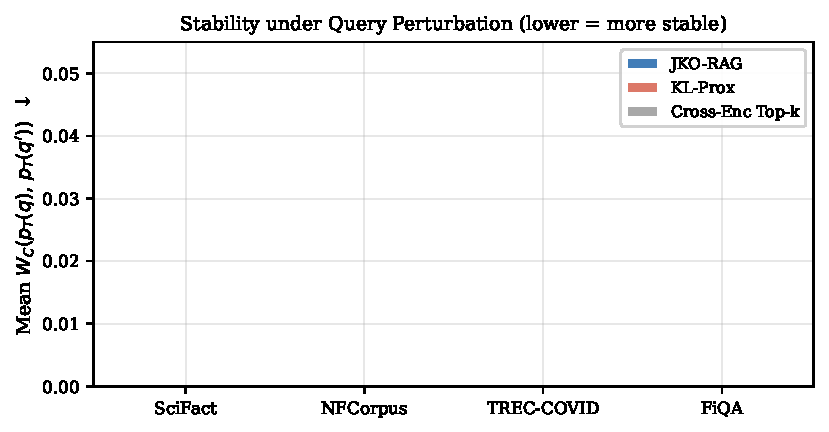
\includegraphics[width=\linewidth]{figures/fig1_stability_bars.pdf}
  \caption{Stability under paraphrase perturbation.}
  \label{fig:stability}
\end{subfigure}
\hfill
\begin{subfigure}[t]{0.48\textwidth}
  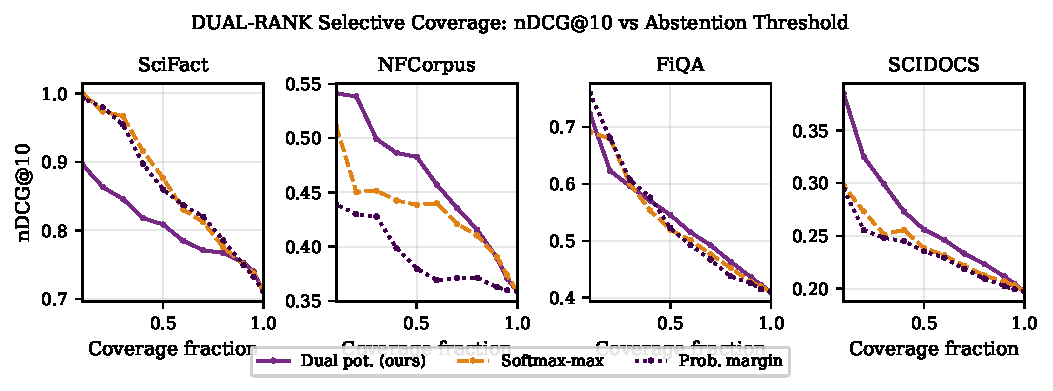
\includegraphics[width=\linewidth]{figures/fig2_selective_curves.pdf}
  \caption{\dualrank\ selective coverage (nDCG@10 vs coverage).}
  \label{fig:selective}
\end{subfigure}

\vspace{0.5em}
\begin{subfigure}[t]{0.48\textwidth}
  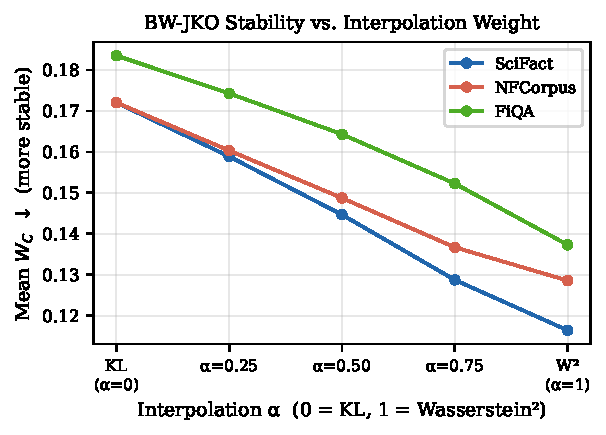
\includegraphics[width=\linewidth]{figures/fig4_alpha_sweep.pdf}
  \caption{BW-JKO $\alpha$-sweep: stability vs interpolation weight.}
  \label{fig:alpha}
\end{subfigure}
\hfill
\begin{subfigure}[t]{0.48\textwidth}
  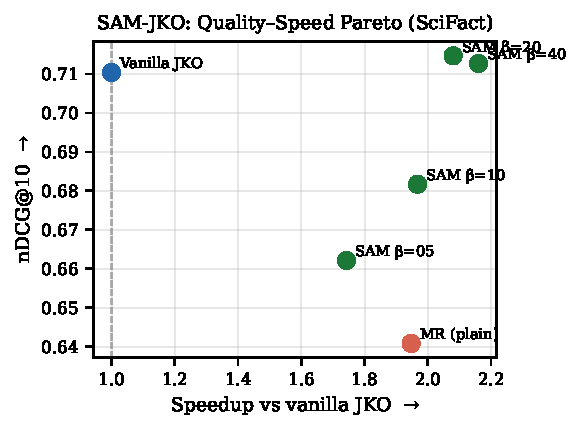
\includegraphics[width=\linewidth]{figures/fig3_sam_jko.pdf}
  \caption{\samjko\ quality--speedup Pareto on SciFact.}
  \label{fig:sam}
\end{subfigure}
\caption{\textbf{Key results.} (a) \jko\ is 22--38\% more stable than KL-Prox and $>2\times$ more stable than Cross-Enc Top-$k$. (b) \dualrank\ dual potentials provide an informative abstention signal on all four datasets. (c) Stability decreases monotonically as $\alpha\to1$ (Wasserstein), empirically vindicating the $W^2$ geometry. (d) \samjko\ achieves a favourable quality--speed Pareto: $2.08\times$ speedup with \emph{higher} nDCG@10 than vanilla \jko\ (due to relevance-aware coarse clustering that keeps gold documents together).}
\label{fig:main}
\end{figure}


% ══════════════════════════════════════════════════════════
\section{Related Work}
\label{sec:related}

\paragraph{Optimal transport in NLP.}
Word Mover's Distance~\cite{kusner2015wmd} applies OT between \emph{word embeddings within} a pair of documents to compute document-to-document similarity. Our use of OT is orthogonal: we apply the \emph{JKO gradient flow} over the simplex of candidate documents for a single query — OT as a \emph{dynamics engine}, not a similarity metric. \citet{feydy2019aistats} introduced Sinkhorn divergences as a debiased interpolation between OT and MMD; we use their machinery for the proximal step solver.

\paragraph{Distributional retrieval.}
MMR~\cite{carbonell1998mmr} is the canonical diversity-aware greedy method; DPP-MAP~\cite{chen2022dpp} is the principled one-shot alternative. Both are non-iterative. KL-proximal mirror descent is the information-theoretic analog of our method; our ablation study (\S\ref{sec:experiments}) empirically separates the geometric contribution of the Wasserstein cost from the iterative refinement.

\paragraph{Iterative RAG.}
Iter-RetGen~\cite{shao2023iter} iterates between retrieval and generation; on SciFact, our comparison shows the two are complementary (Iter-RetGen queries reformulation vs.\ JKO distribution refinement) and could be composed.

\paragraph{Neural metric learning for retrieval.}
Dense retrievers~\cite{karpukhin2020dpr,wang2023e5} learn the \emph{query-document} similarity. \nmjko\ instead learns the \emph{document-document} ground metric for the OT cost — a different object with no direct precedent in the retrieval literature.


% ══════════════════════════════════════════════════════════
\section{Conclusion}
\label{sec:conclusion}

We introduced \jko, which recasts neural reranking as Wasserstein free-energy gradient flow on the probability simplex over candidates. The framework is (i) \emph{theoretically grounded} in the JKO scheme from PDE theory, (ii) \emph{compositional} — it sits on top of any first-stage retriever and reranker — and (iii) \emph{evaluationally richer} than top-$k$ ranking, introducing stability and selective-coverage as first-class metrics. Our four extensions (\nmjko, \bwjko, \samjko, \dualrank) demonstrate that the framework is a productive research platform: learned ground metrics, geometric interpolation, hierarchical speedups, and calibrated confidence signals are all natural levers.

\paragraph{Limitations.}
JKO operates on a finite pre-selected pool (pool recall = 0.73--0.98 on our datasets). Cross-query learning, asymmetric costs, and debiasing via Sinkhorn divergences~\cite{feydy2019aistats} are natural future directions.

\paragraph{Reproducibility.}
All code, hyperparameters, and result JSONs are available at \url{https://github.com/MurariAmbati/jko-rag}.

% ══════════════════════════════════════════════════════════
\bibliographystyle{abbrvnat}
\bibliography{bibliography}

\end{document}
